\documentclass[landscape,a0paper,fontscale=0.4]{baposter}
% make fontscale bigger to get smaller fonts

\tracingstats=2

\usepackage{times}
\usepackage{calc}
\usepackage{url}
\usepackage{graphicx}
\usepackage{amsmath}
\usepackage{amssymb}
\usepackage{relsize}
\usepackage{multirow}
\usepackage{caption}
% \usepackage[authoryear,round]{natbib}
\usepackage[hidelinks]{hyperref}
\usepackage{booktabs}

\usepackage{graphicx}
\usepackage{multicol}
\usepackage[T1]{fontenc}
\usepackage{ae}

\usepackage{minted}
\setminted{fontsize=\scriptsize}

\graphicspath{{images/}}

 %%%%%%%%%%%%%%%%%%%%%%%%%%%%%%%%%%%%%%%%%%%%%%%%%%%%%%%%%%%%%%%%%%%%%%%%%%%%%%%%
 %%%% Some math symbols used in the text
 %%%%%%%%%%%%%%%%%%%%%%%%%%%%%%%%%%%%%%%%%%%%%%%%%%%%%%%%%%%%%%%%%%%%%%%%%%%%%%%%
 % Format 
\newcommand{\R}{\mathbb{R}}
\newcommand{\E}{\mathbb{E}}
\renewcommand{\P}{\mathbb{P}}
\newcommand{\st}{\,\colon\,}
\newcommand{\bone}{\mathbf{1}}
\newcommand{\var}{\mathop{\mbox{Var}}}
\newcommand{\cov}{\mathop{\mbox{cov}}}
\newcommand{\tskit}{{\texttt{tskit}}}
\newcommand{\branch}{\mbox{Branch}} % branch stat
\newcommand{\branchp}{\mbox{Branch}_+} % polarised
\newcommand{\site}{\mbox{Site}} % site stat
\newcommand{\sitep}{\mbox{Site}_+} % polarised
\newcommand{\node}{\mbox{Node}} % node stat
\newcommand{\nodep}{\mbox{Node}_+} % polarised
\newcommand{\given}{\;\vert\;}


 %%%%%%%%%%%%%%%%%%%%%%%%%%%%%%%%%%%%%%%%%%%%%%%%%%%%%%%%%%%%%%%%%%%%%%%%%%%%%%%%
 % Multicol Settings
 %%%%%%%%%%%%%%%%%%%%%%%%%%%%%%%%%%%%%%%%%%%%%%%%%%%%%%%%%%%%%%%%%%%%%%%%%%%%%%%%
 \setlength{\columnsep}{0.7em}
 \setlength{\columnseprule}{0mm}


 %%%%%%%%%%%%%%%%%%%%%%%%%%%%%%%%%%%%%%%%%%%%%%%%%%%%%%%%%%%%%%%%%%%%%%%%%%%%%%%%
 % Save space in lists. Use this after the opening of the list
 %%%%%%%%%%%%%%%%%%%%%%%%%%%%%%%%%%%%%%%%%%%%%%%%%%%%%%%%%%%%%%%%%%%%%%%%%%%%%%%%
 \newcommand{\compresslist}{%
 \setlength{\itemsep}{1pt}%
 \setlength{\parskip}{0pt}%
 \setlength{\parsep}{0pt}%
 }

%%%%%%%%%%%%%%%%%%%%%%%%%%%%%%%%%%%%%%%%%%%%%%%%%%%%%%%%%%%%%%%%%%%%%%%%%%%%%%
%%% Other Macros
%%%%%%%%%%%%%%%%%%%%%%%%%%%%%%%%%%%%%%%%%%%%%%%%%%%%%%%%%%%%%%%%%%%%%%%%%%%%%%
% \renewcommand{\labelenumi}{\alph{enumi})}
% \renewcommand{\theenumi}{\alph{enumi})}
\newcommand{\postercaption}[1]{\begin{minipage}{\linewidth}\center\smaller
  {#1}\end{minipage}}



%%%%%%%%%%%%%%%%%%%%%%%%%%%%%%%%%%%%%%%%%%%%%%%%%%%%%%%%%%%%%%%%%%%%%%%%%%%%%
%% Begin of Document
%%%%%%%%%%%%%%%%%%%%%%%%%%%%%%%%%%%%%%%%%%%%%%%%%%%%%%%%%%%%%%%%%%%%%%%%%%%%%
\begin{document}

% Define some colors
\definecolor{tskitMint}{RGB}{93,199,148}  % 5dc794
\definecolor{tskitBlue}{RGB}{31,78,102}  % 1f4e66

\definecolor{silver}{cmyk}{0,0,0,0.3}
\definecolor{black}{cmyk}{0,0,0.0,1.0}
\definecolor{white}{cmyk}{0,0,0.0,0.0}
\definecolor{darkSilver}{cmyk}{0,0,0,0.1}

\definecolor{darkYellow}{cmyk}{0,0,1.0,0.5}
\definecolor{yellow}{cmyk}{0,0,0.9,0.0}
\definecolor{reddishyellow}{cmyk}{0,0.22,1.0,0.0}
\definecolor{lightyellow}{cmyk}{0,0,0.3,0.0}
\definecolor{lighteryellow}{cmyk}{0,0,0.1,0.0}
\definecolor{lightestyellow}{cmyk}{0,0,0.05,0.0}

\definecolor{darkCyan}{cmyk}{1,1,0,0.5}
\definecolor{cyan}{cmyk}{1,0,0,0.0}
\definecolor{lightcyan}{cmyk}{0.3,0,0,0.0}
\definecolor{lightercyan}{cmyk}{0.1,0,0,0.0}
\definecolor{lightestcyan}{cmyk}{0.05,0,0,0.0}

%%%%%%%%%%%%%%%%%%%%%%%%%%%%%%%%%%%%%%%%%%%%%%%%%%%%%%%%%%%%%%%%%%%%%%%%%%%%%
%% Here starts the poster
%%---------------------------------------------------------------------------
%% Format it to your taste with the options
%%%%%%%%%%%%%%%%%%%%%%%%%%%%%%%%%%%%%%%%%%%%%%%%%%%%%%%%%%%%%%%%%%%%%%%%%%%%%
\begin{poster}{
 % Show grid to help with alignment
 grid=false,
 % Column spacing
 colspacing=0.7em,
 % Color style
 headerColorOne=tskitMint,
 borderColor=tskitBlue,
 % Format of textbox
 textborder=faded,
 % Format of text header
 headerborder=open,
 headershape=roundedright,
 headershade=plain,
 background=none,
 bgColorOne=tskitMint,
 headerheight=0.12\textheight}
 % Eye Catcher
 { \includegraphics[height=0.12\textheight]{tskit_logo}
 }
 % Title
{\resizebox{0.95\textwidth}{!}{\Huge \tskit{}: \sc population-scale genomics and phylogenetics}}
 % Authors
  {\sf %Sans Serif
    Ben Jeffery${}^\ddagger$,
    Jerome Kelleher$^{\ddagger}$,
    Nathaniel Pope${}^\dagger$,
    Peter Ralph${}^\dagger$,
    \\  \vspace{-1.0mm}
    Georgia Tsambos,${}^{\dagger\S}$,
    Yan Wong$^{\ddagger}$,
    and the rest of the tskit-dev group.
    \\  \vspace{-1.0mm}
    Code: \url{github.com/petrelharp/progen-2023}. 
    \\  \vspace{-1.0mm}
    {\small \textit{$\dagger$ University of Oregon} } %\\ \vspace{-0.5em}
    {\small \textit{$\ddagger$ University of Oxford} } %\\ \vspace{-0.5em}
    {\small \textit{$\S$ University of Washington}} \\
  }
 % University logo
 {
  \begin{tabular}{r}
    \includegraphics[height=0.12\textheight]{oxford-logo.jpeg}
      \hspace{1em}
    \includegraphics[height=0.12\textheight]{UOSignature-STK-BLK}\\
  \end{tabular}
 }

%%%%%%%%%%%%%%%%%%%%%%%%%%%%%%%%%%%%%%%%%%%%%%%%%%%%%%%%%%%%%%%%%%%%%%%%%%%%%%
%%% Now define the boxes that make up the poster
%%%---------------------------------------------------------------------------
%%% Each box has a name and can be placed absolutely or relatively.
%%% The only inconvenience is that you can only specify a relative position 
%%% towards an already declared box. So if you have a box attached to the 
%%% bottom, one to the top and a third one which should be inbetween, you 
%%% have to specify the top and bottom boxes before you specify the middle 
%%% box.
%%%%%%%%%%%%%%%%%%%%%%%%%%%%%%%%%%%%%%%%%%%%%%%%%%%%%%%%%%%%%%%%%%%%%%%%%%%%%%

%%%%%%%%%%%%%%%%%%%%%%%%%%%%%%%%%%%%%%%%%%%%%%%%%%%%%%%%%%%%%%%%%%%%%%%%%%%%%%
\begin{posterbox}[name=inout,column=0,span=1,above=bottom]{Metadata}
%%%%%%%%%%%%%%%%%%%%%%%%%%%%%%%%%%%%%%%%%%%%%%%%%%%%%%%%%%%%%%%%%%%%%%%%%%%%%%

    \tskit{} now has integrated metadata
    for all objects (genomes, mutations, sites, etc).
    For instance \emph{(spoiler alert)},
    the complete ARG for 1.26 million SARS-Cov-2 genomes (until mid-2021):
    fits in 57MB, and loads in under 1 second!
    It is 819 MB once decompressed, and has metadata attached to three tables.

% \begin{minted}{bash}
% ls -lh SARS-Cov-2-ARG.ts.tsz
% \end{minted}
{\scriptsize \verb|-rw-rw-r-- 1 jk jk 57M Mar  2 13:32 SARS-Cov-2-ARG.ts.tsz|}
\begin{minted}{python}
ts = tszip.decompress("SARS-Cov-2-ARG.ts.tsz")
\end{minted}
{\scriptsize
\begin{verbatim}
CPU times: user 775 ms, sys: 533 ms, total: 1.31 s
Wall time: 842 ms
\end{verbatim}
}
\begin{center}
    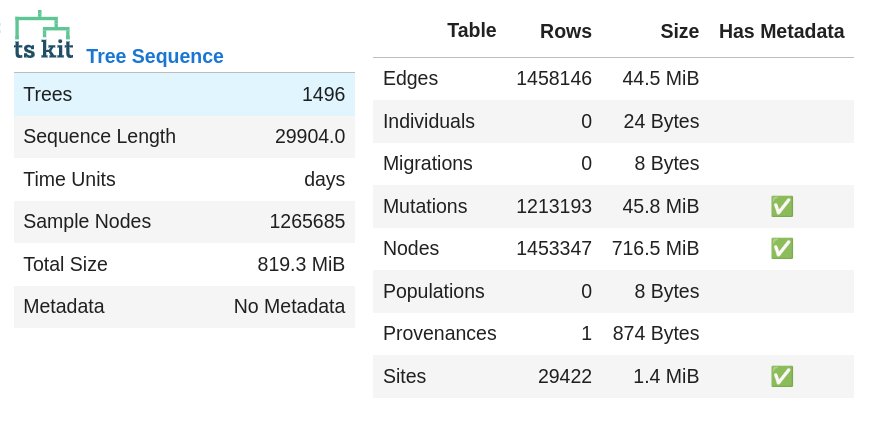
\includegraphics[width=0.5\textwidth]{sc2_ts.png}
\end{center}

\paragraph{The integrated data model}
links nodes, edges, sites and mutations,
and now allows annotation of all objects with arbitrary external metadata.
For instance,
here's the first five sites in the SARS-Cov-2 ARG,
and
% all three mutations at the first site:
    metadata for a sample (available as a dictionary!):

\begin{multicols}{2}
\begin{minted}{python}
ts.tables.sites[:5]
\end{minted}
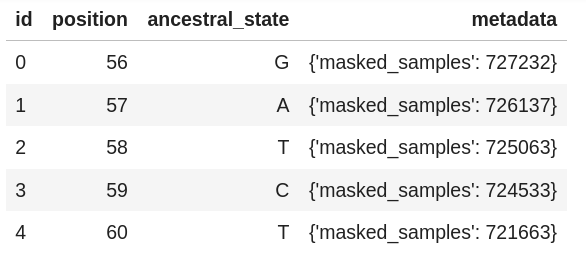
\includegraphics[width=0.5\textwidth]{sc2_sites}

    \vspace{2em}

% \begin{minted}{python}
% ts.tables.mutations[ts.mutations_site == 0]
% \end{minted}
% 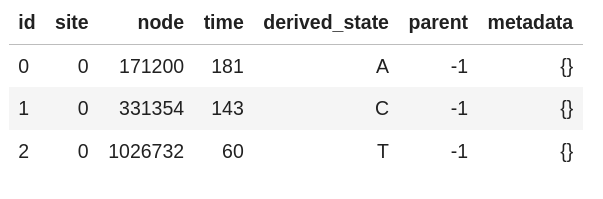
\includegraphics[width=0.5\textwidth]{sc2_muts}
\columnbreak
% All the information \tskit{} knows about can be accessed
% as dictionaries.
% Here's one of the samples:
% 
\tiny
\begin{minted}{python}
dataclasses.asdict(ts.node(1026732))
\end{minted}
\tiny
\begin{minted}{python}
{'id': 1026732, 'flags': 1, 'time': 60.0,
 'metadata': {'Imputed_lineage': 'B.1.1.7',
  'Nextclade_pango': 'B.1.1.7',
  'clade': '20I (Alpha, V1)',
  'country': 'Germany', 'date': '2021-05-01',
  'date_submitted': '2021-05-17',
  'gisaid_epi_isl': 'EPI_ISL_2122637',
  'sc2ts_qc': {'num_masked_sites': 150,
   'original_base_composition': {'-': 103,
    'A': 8902, 'C': 5473, 'G': 5847, 'T': 9578}},
  'strain': 'Germany/un-RKI-I-137988/2021',
  'totalSubstitutions': 36.0}}
\end{minted}

\end{multicols}

\end{posterbox}
%%%%%%%%%%%%%%%%%%%%%%%%%%%%%%%%%%%%%%%%%%%%%%%%%%%%%%%%%%%%%%%%%%%%%%%%%%%%%%

%%%%%%%%%%%%%%%%%%%%%%%%%%%%%%%%%%%%%%%%%%%%%%%%%%%%%%%%%%%%%%%%%%%%%%%%%%%%%%
\begin{posterbox}[name=interop,column=0,row=0,span=1]{Interfaces and interoperability}
%%%%%%%%%%%%%%%%%%%%%%%%%%%%%%%%%%%%%%%%%%%%%%%%%%%%%%%%%%%%%%%%%%%%%%%%%%%%%%


We aim to provide \emph{stable}, \emph{well-tested} and \emph{well-documented}
software so others can reliably build with it --
including a \emph{backwards compatibility} guarantee.
\tskit{} is already being used in a number of inference and simulation packages.
The core functionality is implemented via a C API,
and the primary interface is via a Python library,
but others are available:

\begin{itemize} \compresslist
    \item Well-tested API used by many software packages: SLiM, fwdpy11, msprime, tsinfer/tsdate, Relate, slendr, etc.
    \item Available in multiple programming languages: \\
        \includegraphics[height=2em]{C_Logo}
        \includegraphics[height=2em]{python-logo-master-v3-TM-flattened}
        \includegraphics[height=2em]{RustLogo}
        
\includegraphics[height=2em]{R-logo}
    \item Runs in-browser (no install required!) for quick demos / teaching (see screenshot).
    \item Can represent full Ancestral Recombination Graphs; includes ARG likelihood calculations.
    \item Interoperable with other packages (e.g., VCF output for sequence data, newick/nexus output to Dendropy, numpy arrays to scikit-allel)
\end{itemize}

% \begin{minted}{python}
% ts = msprime.sim_ancestry(2, sequence_length=600,
%         recombination_rate=1e-3, random_seed=7)
% ts = msprime.sim_mutations(ts, rate=2e-3, random_seed=9)
% 
% css = (".tree .plotbox {transform: skewY(0.7rad) "
%         "translateY(-50px)}")
% ts.draw_svg(size=(700, 200), x_scale="treewise",
%         style=css, mutation_labels={})
% \end{minted}

    \begin{center}
    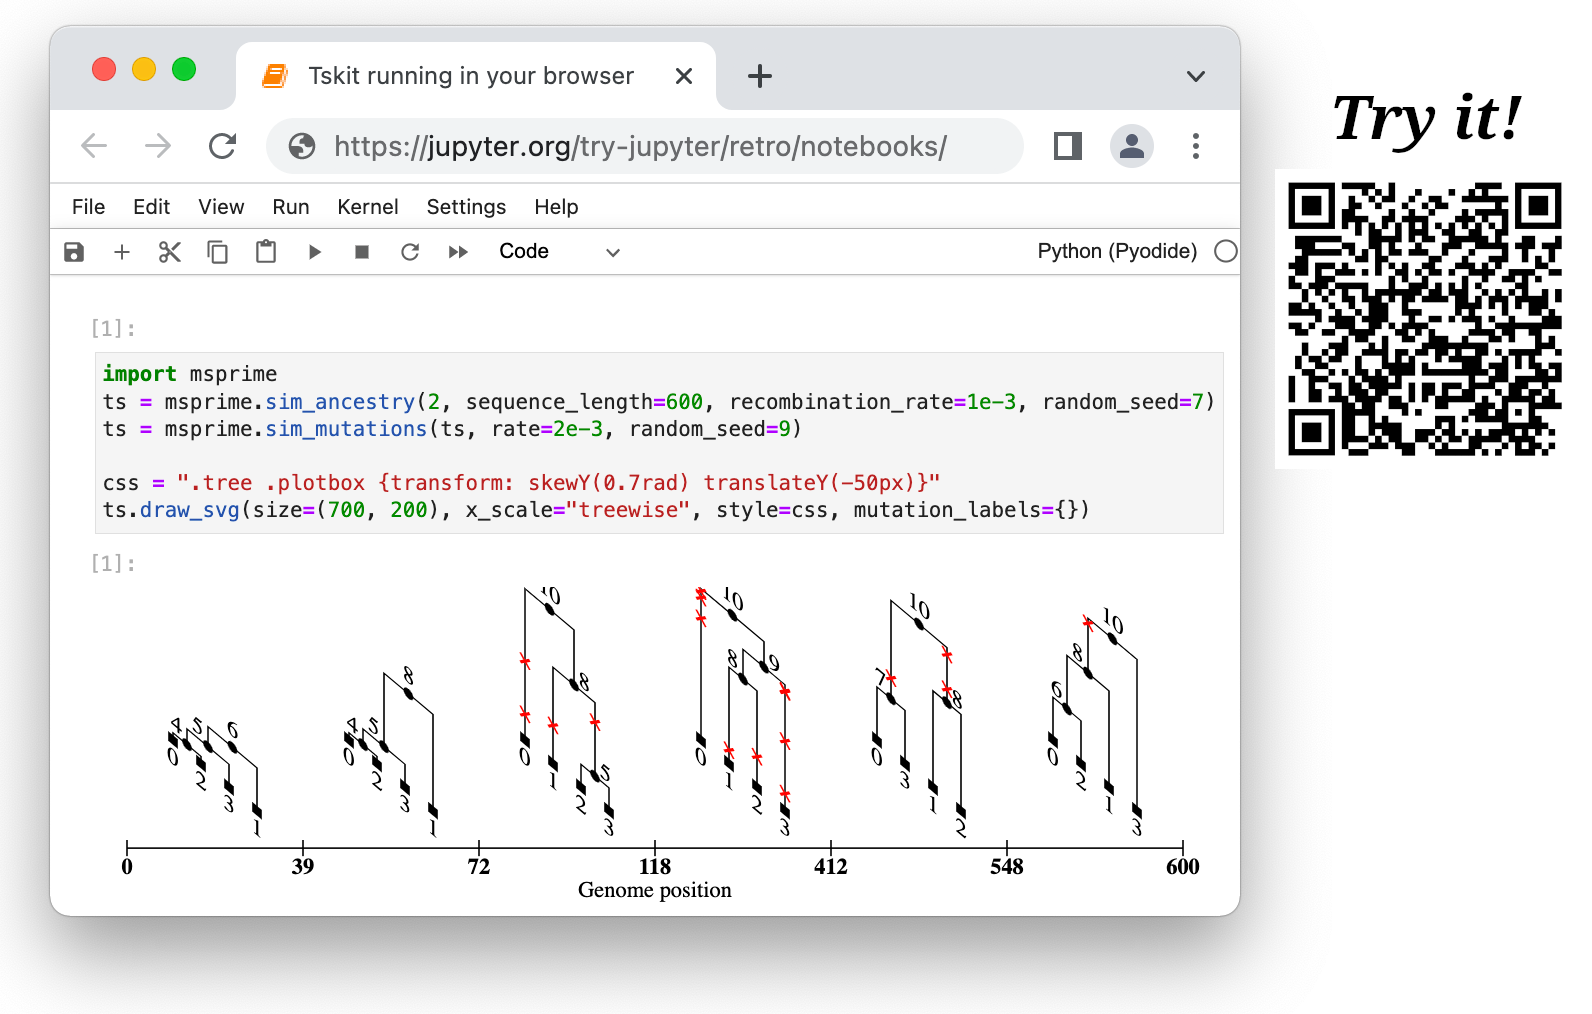
\includegraphics[width=0.7\textwidth]{JupyterLite_plus_qr}
    \end{center}


\end{posterbox}
%%%%%%%%%%%%%%%%%%%%%%%%%%%%%%%%%%%%%%%%%%%%%%%%%%%%%%%%%%%%%%%%%%%%%%%%%%%%%%

%%%%%%%%%%%%%%%%%%%%%%%%%%%%%%%%%%%%%%%%%%%%%%%%%%%%%%%%%%%%%%%%%%%%%%%%%%%%%%
\begin{posterbox}[name=overview,column=1,row=0,span=2]{Overview}
%%%%%%%%%%%%%%%%%%%%%%%%%%%%%%%%%%%%%%%%%%%%%%%%%%%%%%%%%%%%%%%%%%%%%%%%%%%%%%

\begin{multicols}{2}

\tskit{} is the C and python library providing tools for working with \emph{succinct tree sequences}.
We provide solid, stable, well-tested software for you to use and build on.
Why might you want to use tree sequences?
\begin{itemize} \compresslist
    \item For large samples,
        stores genotypes losslessly using (estimated) underlying genealogical relationships
        in orders of magnitude less space,
    \item \ldots and allows fast processing and exploration, in seconds, not hours.
    \item Genealogical relationships -- ``the trees'' -- are often closer to
        things we want to learn about
    \item \ldots and explicitly include a \emph{time dimension}.
    \item History of a process can be recorded in a simulation, not just the genotypic outcome,
    \item \ldots and simulations can be much faster/more efficient.
\end{itemize}

In summary:
by representing genomes using the genealogical process that generated the data,
we get both a huge advantage storing and manipulating genomic data,
as well as a more direct look at the processes that generated the data.

    \vspace{2em}

Here's some \textbf{silly slogans}, care to suggest any more?
\begin{itemize} \compresslist
    \item ``\tskit: launching your genomes into the time dimension!''
    \item ``\tskit: tree thinking, for popgen''
    \item ``\tskit: stable software for genome-scale trees''
    \item ``\tskit: all your insights, much faster!''
\end{itemize}

\end{multicols}

\begin{center} \Large
    Documentation and examples: \url{https://tskit.dev/}

    \vspace{2em}

    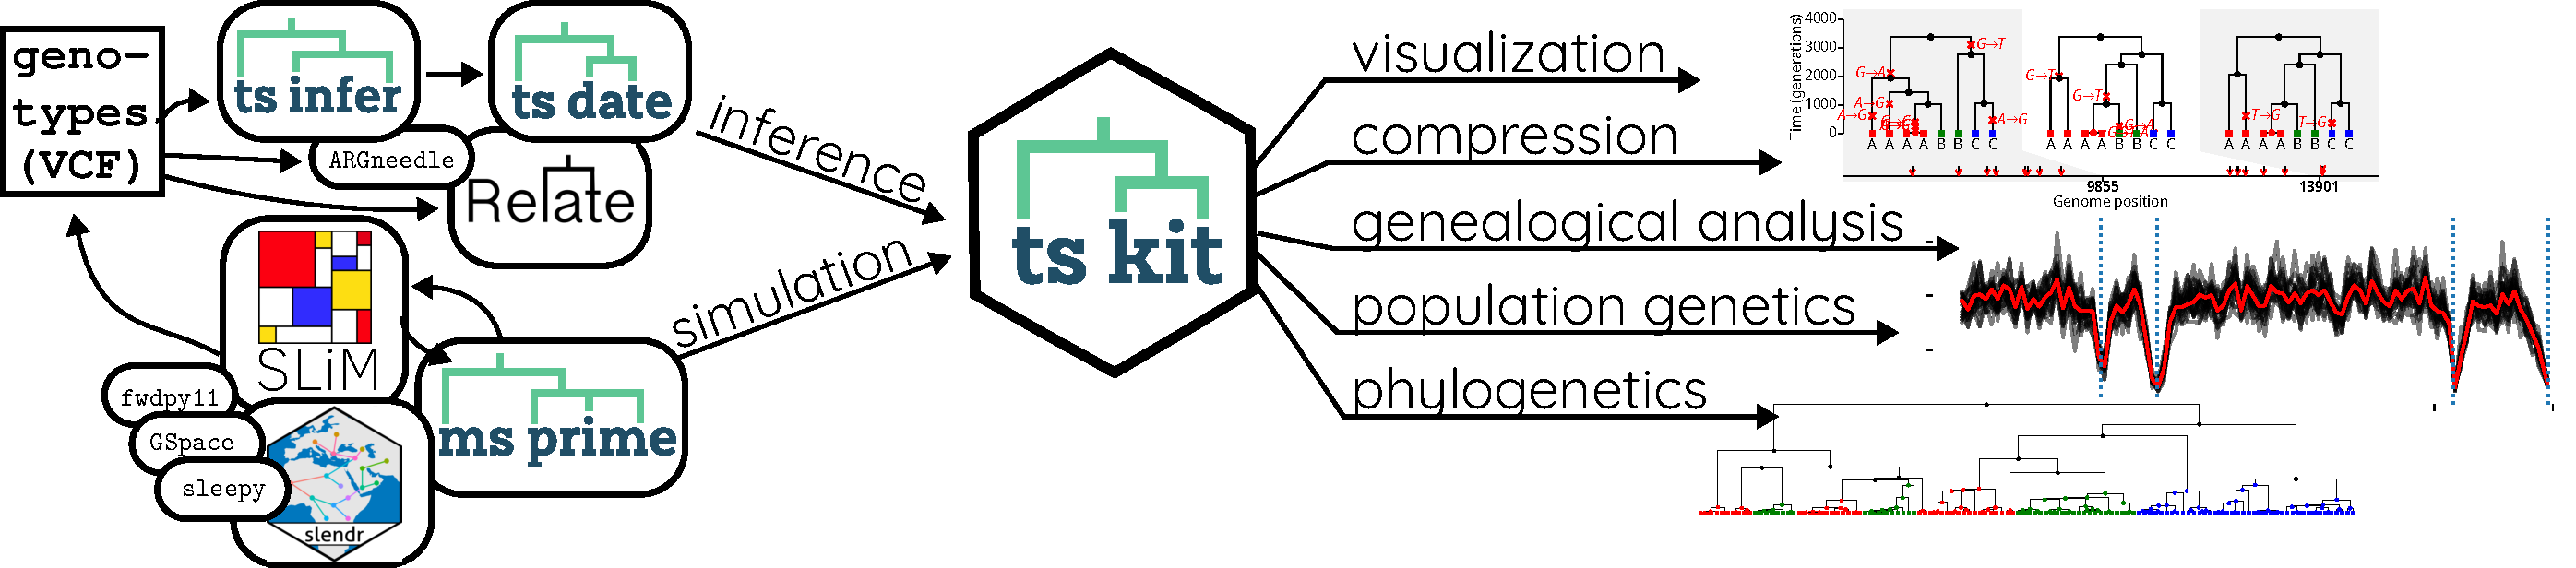
\includegraphics[width=0.85\textwidth]{workflow}
\end{center}


\end{posterbox}
%%%%%%%%%%%%%%%%%%%%%%%%%%%%%%%%%%%%%%%%%%%%%%%%%%%%%%%%%%%%%%%%%%%%%%%%%%%%%%

%%%%%%%%%%%%%%%%%%%%%%%%%%%%%%%%%%%%%%%%%%%%%%%%%%%%%%%%%%%%%%%%%%%%%%%%%%%%%%
\begin{posterbox}[name=viz,column=1,row=0,span=2,below=overview]{Visuzalization -- \textup{see more at \url{https://tskit.dev/tutorials/viz.html}}}
%%%%%%%%%%%%%%%%%%%%%%%%%%%%%%%%%%%%%%%%%%%%%%%%%%%%%%%%%%%%%%%%%%%%%%%%%%%%%%


\begin{multicols}{2}

SVG-based visualization allows flexible styling of local trees.

\begin{itemize} \compresslist
    \item set labels for nodes, mutations, and tickmarks: e.g., using metadata
    \item color elements: e.g., to highlight branches that change between trees,
        mutations by type, or samples by location
    \item transform elements: e.g., rotate labels, alter node symbols, even 3D effects!
    \item timescale titles show time units by default (scaling can be linear, log, or rank)
    \item interaction possible via mouseover events and javascript animation
    \item text-based plots also available for simple debugging
\end{itemize}

\begin{center}
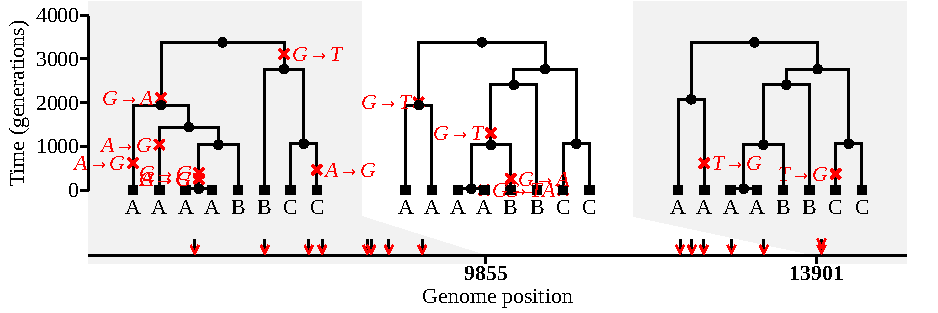
\includegraphics[width=0.5\textwidth]{viz_23_0}
\end{center}

% \begin{minted}{python}
% simp_ts.draw_svg(
%     size=(800, 400),
%     canvas_size=(850, 405),
%     style=style + "".join(node_styles),
%     y_axis=True,
%     time_scale="log_time",
%     symbol_size=4.5,
%     y_label = "Date",
%     x_label = "SARS-CoV-2 genome position",
%     y_ticks = y_ticks,
%     mutation_labels={},
%     y_gridlines=True,
%     node_labels=node_labels,
%     root_svg_attributes={"id": "ns_rec"},
% )
% \end{minted}

\columnbreak
\paragraph{Example:}
SARS-CoV-2 samples affected by recombination, subset from a 1.2M
sample Covid tree sequence
\begin{minted}{python}
simp_ts.draw_svg(
    size=(800, 400), canvas_size=(850, 405),
    style=style + "".join(node_styles),
    y_axis=True, time_scale="log_time",
    symbol_size=4.5, y_label = "Date",
    x_label = "SARS-CoV-2 genome position",
    y_ticks = y_ticks, mutation_labels={},
    y_gridlines=True, node_labels=node_labels,
    root_svg_attributes={"id": "ns_rec"},
)
\end{minted}

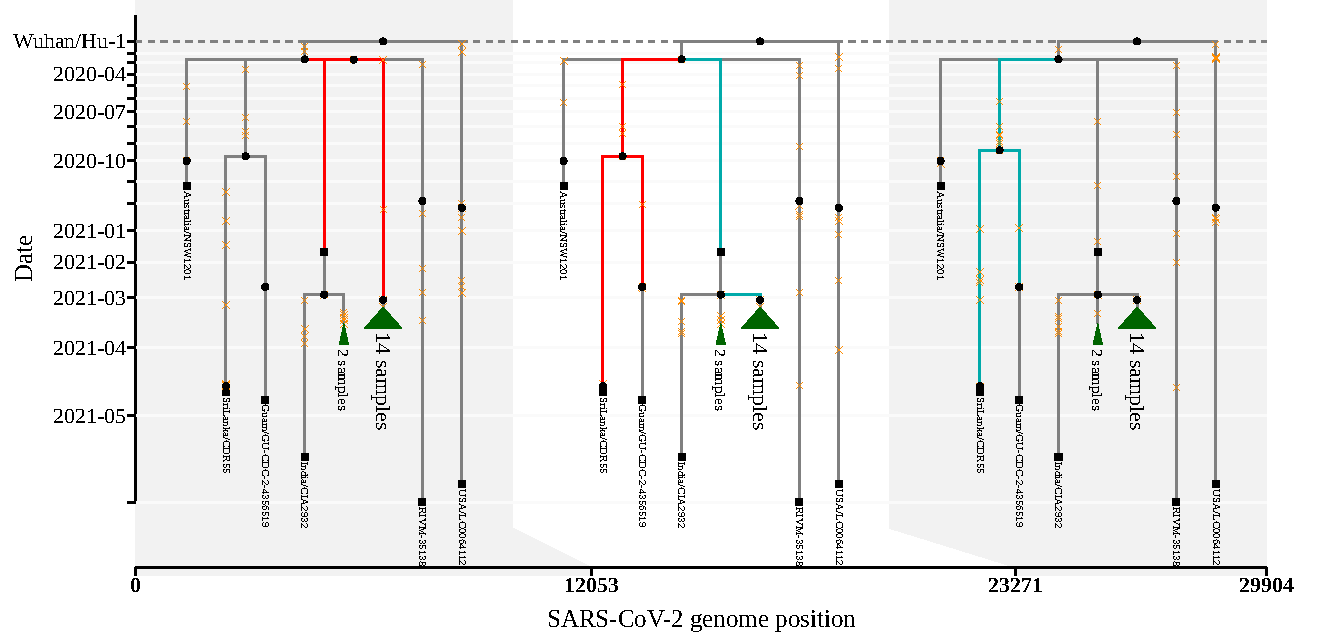
\includegraphics[width=0.5\textwidth]{Covid_recombination}

\end{multicols}

\end{posterbox}
%%%%%%%%%%%%%%%%%%%%%%%%%%%%%%%%%%%%%%%%%%%%%%%%%%%%%%%%%%%%%%%%%%%%%%%%%%%%%%



%%%%%%%%%%%%%%%%%%%%%%%%%%%%%%%%%%%%%%%%%%%%%%%%%%%%%%%%%%%%%%%%%%%%%%%%%%%%%%
\begin{posterbox}[name=stats,column=3,row=0,span=1]{Statistics}
%%%%%%%%%%%%%%%%%%%%%%%%%%%%%%%%%%%%%%%%%%%%%%%%%%%%%%%%%%%%%%%%%%%%%%%%%%%%%%

\tskit{} lets you perform efficient calculations of statistics along the genome, often many times quicker than other software! You may be interested in calculating:

\begin{itemize} \compresslist
    \item the allele frequency spectrum or statistics derived from it,
        like nucleotide diversity, Tajima's $D$, f4, \ldots
    \item IBD-based quantities,
    \item summaries of tree topology,
        e.g., genealogical nearest neighbours and tree balance metrics,
    \item cross-coalescence rates (coming soon!)
\end{itemize}

\paragraph{Example:} newly-implemented tree balance statistics. A balanced
(binary) tree is perfectly symmetric in some way: each node's
subtrees are of equal size, where `size'
is determined by some metric involving the tree's nodes and edges. \tskit{}
now implements several different metrics of balance:

\begin{minted}{python}
imb = pd.DataFrame({
    "genomic position" : [t.interval[0] for t in ts.trees()],
    "b1" : [t.b1_index() for t in ts.trees()],
    "b2" : [t.b2_index() for t in ts.trees()],
    "colless" : [t.colless_index() for t in ts.trees()],
    "sackin" : [t.sackin_index() for t in ts.trees()]
}).set_index("genomic position")

imb = ((imb - imb.mean()) / imb.std())
imb.plot(figsize=(16, 4), alpha=0.7)
\end{minted}
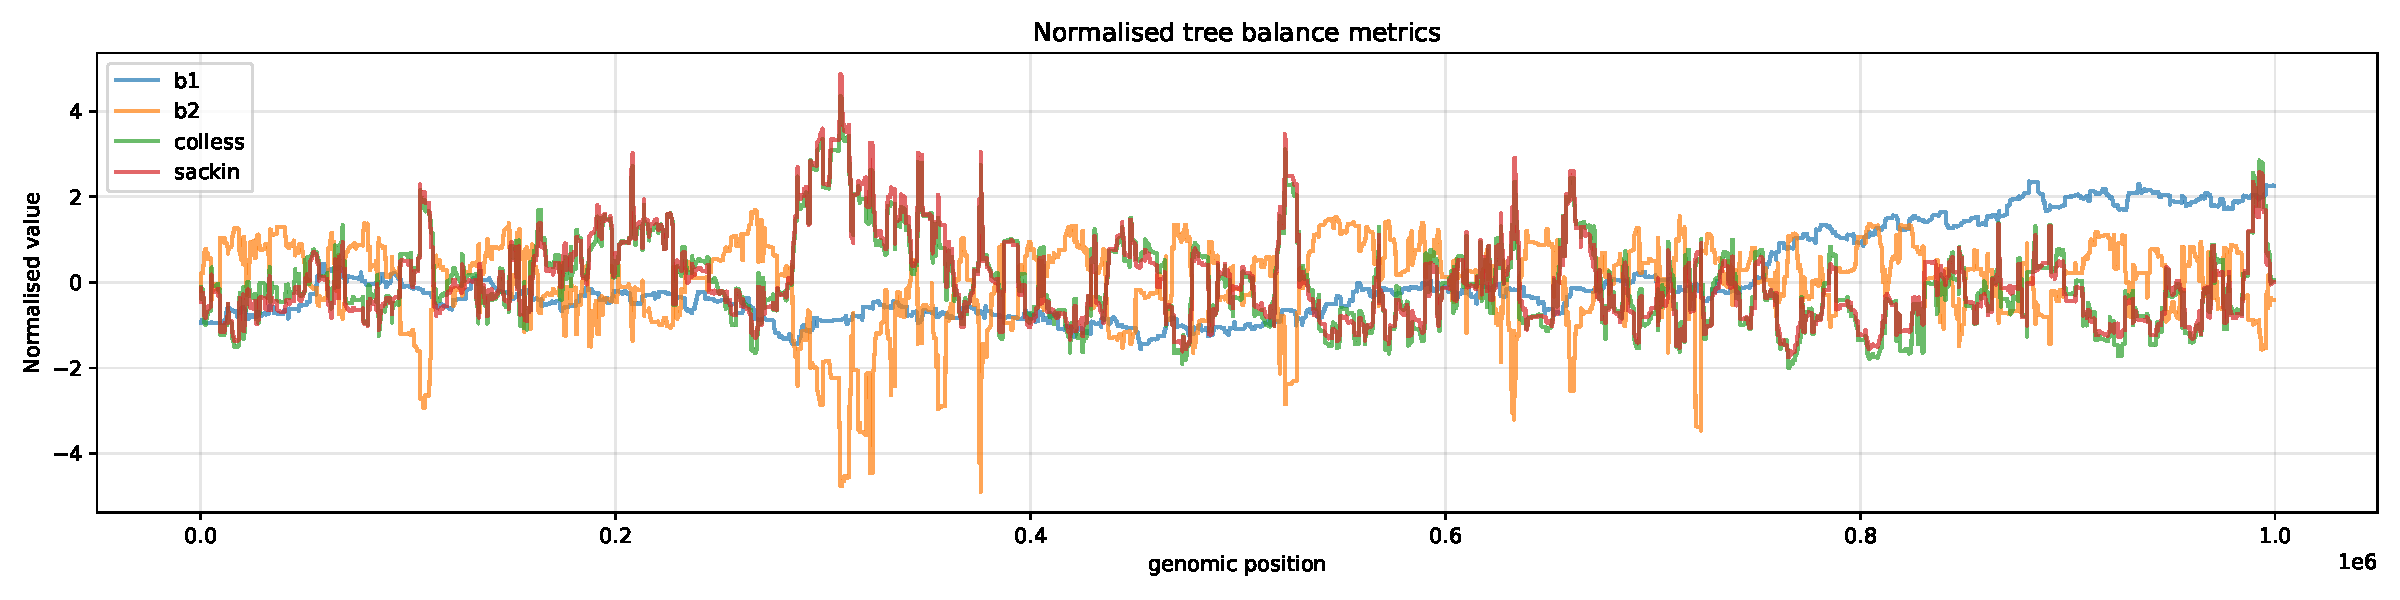
\includegraphics[width=\textwidth]{tree_balance}

\end{posterbox}
%%%%%%%%%%%%%%%%%%%%%%%%%%%%%%%%%%%%%%%%%%%%%%%%%%%%%%%%%%%%%%%%%%%%%%%%%%%%%%


%%%%%%%%%%%%%%%%%%%%%%%%%%%%%%%%%%%%%%%%%%%%%%%%%%%%%%%%%%%%%%%%%%%%%%%%%%%%%%
\begin{posterbox}[name=operations,column=3,above=bottom,span=1]{Notable new features}
%%%%%%%%%%%%%%%%%%%%%%%%%%%%%%%%%%%%%%%%%%%%%%%%%%%%%%%%%%%%%%%%%%%%%%%%%%%%%%

    % \emph{Example notebook: \url{https://github.com/petrelharp/progen-2023/new-features.ipynb}}

\tskit{}'s contributors are actively working on
    new features, bug fixes, and improvements to the usability of existing
    features. Here's a shortlist of some recent additions:

\paragraph{Reference sequences}
By default, the sites in a tree sequence only give ancestral state at
    polymorphic sites. Remaining positions can now be specified using the
    \texttt{TreeSequence.reference\_sequence}, and individual sample alignments can
    be obtained with the \texttt{TreeSequence.alignments()} iterator.

\paragraph{Structural operations}
We've expanded the set of utility functions for large edits on tree sequences.
    For instance, the \texttt{TreeSequence.decapitate} method removes all parts of a
    tree sequence that are older than some user-specified time,
    and \texttt{TreeSequence.union} joins together separate tree sequences,
    allowing parallel simulation across different branches of a phylogenetic tree.

\paragraph{Efficient array access}
The relationships between nodes in each tree can now be extracted as \texttt{numpy}
    arrays. When used with \texttt{numba},
    Python-based calculations on the trees can be as fast as
    machine-level code. Here is numba $+$ python computing total branch length
    (see example code)
    just as fast as the ``built-in'' method (implemented in C),
    and 10--100$\times$ faster than the un-numba'ed python code:

\begin{multicols}{2}
\begin{minted}{python}
@numba.njit
def _total_branch_length(order, parent, time):
   tbl = 0
   for u in order:
     if parent[u] != -1:
       tbl += time[parent[u]] - time[u]
   return tbl

def get_total_branch_length(tree):
   return _total_branch_length(
     tree.preorder(), tree.parent_array,
     tree.tree_sequence.nodes_time)
\end{minted}

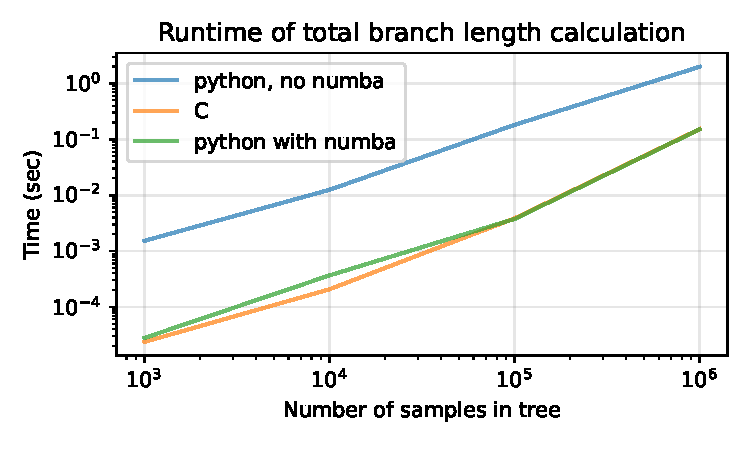
\includegraphics[width=0.5\textwidth]{numba_runtime}
\end{multicols}

\end{posterbox}
%%%%%%%%%%%%%%%%%%%%%%%%%%%%%%%%%%%%%%%%%%%%%%%%%%%%%%%%%%%%%%%%%%%%%%%%%%%%%%



%%%%%%%%%%%%%%%%%%%%%%%%%%%%%%%%%%%%%%%%%%%%%%%%%%%%%%%%%%%%%%%%%%%%%%%%%%%%%%
\begin{posterbox}[name=refs,column=1,span=2,above=bottom]{Contributors}
%%%%%%%%%%%%%%%%%%%%%%%%%%%%%%%%%%%%%%%%%%%%%%%%%%%%%%%%%%%%%%%%%%%%%%%%%%%%%%

\tskit{} is developed by an open and inclusive community.
Want to get involved?
All skill levels welcome -- email us at \url{admin@tskit.dev}.

\begin{center}
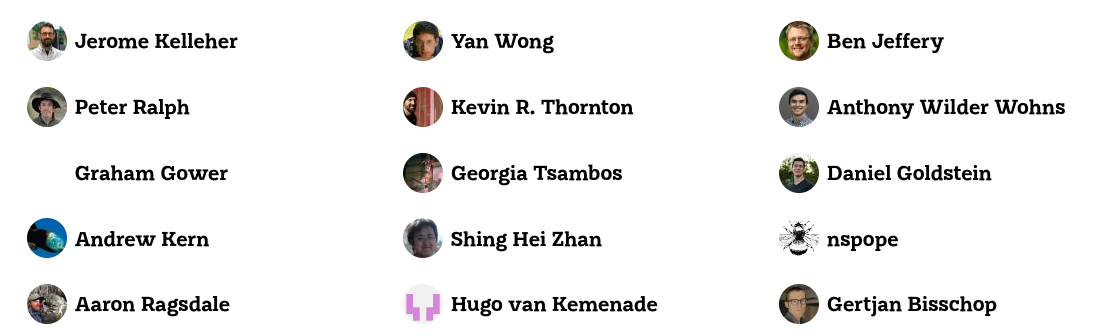
\includegraphics[width=0.47\textwidth]{tskit-contributors1}
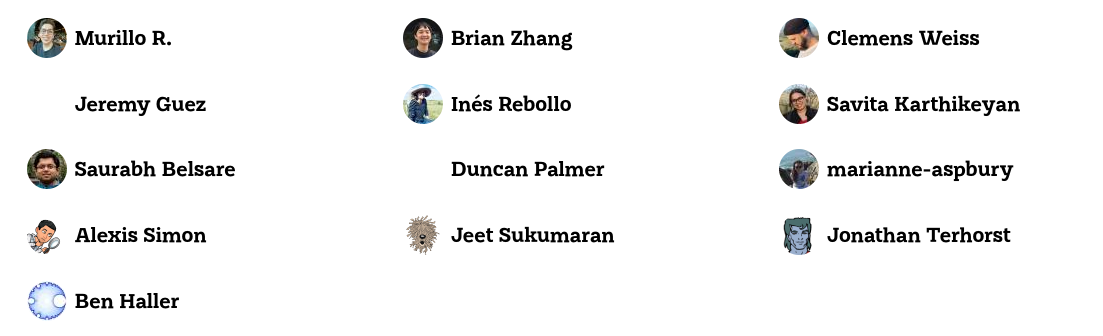
\includegraphics[width=0.47\textwidth]{tskit-contributors2}
\end{center}

  % % \scriptsize
  % \renewcommand{\section}[2]{\vskip 0.0em}
  % \bibliographystyle{abbrvnat}
  % \setlength{\bibsep}{0.0pt}

  % \bibliography{refs}
\end{posterbox}
%%%%%%%%%%%%%%%%%%%%%%%%%%%%%%%%%%%%%%%%%%%%%%%%%%%%%%%%%%%%%%%%%%%%%%%%%%%%%%


\end{poster}%
\end{document}
